\chapter{Implementacion, desarrollo y pruebas comparativas}
\section{Implementación y desarrollo}
Con el objetivo de contar con una nariz electrónica operativa que complemente el trabajo de los agentes caninos, se decidió entrenar una red neuronal artificial (ANN). Esta se integrará en una aplicación Bluetooth para dispositivos móviles que controlará la nariz electrónica. Dicha red neuronal será la encargada de determinar si la muestra analizada corresponde o no a la sustancia objetivo.
\par

La implementación y el desarrollo de la nariz electrónica se estructuran en tres fases:
\begin{itemize}
    \item Construcción del conjunto de datos (dataset).
    \item Entrenamiento de la red neuronal.
    \item Desarrollo de la aplicación móvil para la comunicación Bluetooth con la nariz electrónica.
\end{itemize}

A continuación, se detallan cada una de estas fases.

\subsection{Construcción del dataset}
Para la construcción del conjunto de datos, se llevaron a cabo múltiples experimentos (tomas de muestras) utilizando la nariz electrónica para recopilar datos de diversas muestras. En total se realizaron 76 experimentos, de los cueles los datos son almacenados en ficheros de texto (uno por cada experimento) que contienen las lecturas de los sensores. Estos ficheros se encuentran disponibles en el repositorio del proyecto mencionado en el capítulo de metodología.
\par

Se busca hacer una clasificación binaria, es decir, distinguir entre dos clases, además de que el entrenamiento de la ANN se realice con un conjunto de datos equilibrado. Para ello, se ha dividido el dataset en dos carpetas (``BUENO'' y ``MALO''): una para las muestras positivas (hachís) y otra para las muestras negativas (otras sustancias) respectivamente. Cada carpeta contiene 38 ficheros de texto correspondientes a los experimentos realizados con cada tipo de muestra.
\par

Para asignarle un nombre identificativo a cada experimento, se ha usado la nomenclatura EXP\_X\_Y-Z, donde:

\begin{itemize}
    \item \textbf{EXP:} Es una anrebiatura de ``EXPERIMENTO''.
    \item \textbf{X:} Indica si la muestra pertenece a la calse ``BUENO'' (B) o ``MALO'' (M).
    \item \textbf{Y:} Es un índicie que, en la muestras positivias, sirve para llevar un conteo de los experimentos realizados, mientras que, en las muestras negativas, se aumenta dicho índice cada vez que se cambia de sustancia.
    \item \textbf{Z:} Es un número secuencial que identifica el experimento dentro de cada sustancia. Es usado en las muestras negativas para diferenciar entre experimentos realizados con la misma sustancia bajo distintas condiciones. En las muestras positivas se omite ya que siempre se trabaja con hachís.
\end{itemize}

\subsubsection{Proceso de toma de muestras}
Se trata de un proceso cíclico que consta de dos fases: desorción (toma de aire limpio para limpiar los sensores y establecer la linea base) y adsorción (toma de la muestra).
\par

Para este proyecto se ha buscado recrear situaciones lo más parecidas posibles a una situación real, por ejemplo, un control de carretera. Para ello, se ha establecido un solo ciclo, con una fase de desorción de 120 segundos (dos minutos), para eliminar cualquier posible resto de impureza que haya posido quedar en los sensores, y una fase de adsorción de 300 segundos (cinco minutos).
\par

Para que el aire entre en la carcasa y entre en contacto con los sensores, se conectan tubos flexibles a las entradas de la carcasa. En la entrada de desorción (IM\_D) se conecta a un tubo conectado a un pequeño purificador de aire para que el aire esté limpio. En la entrada de adsorción (IM\_A) se conecta a un tubo que conecta con el bote de muestreo donde estará la sustancia. A su vez, este bote de muestreo también esta conectado a otro purificador de aire para que entre aire limpio en el bote y se cree una corriente de aire, permitiendo que el aire de dentro del bote pueda ser absorbido mas facilmente por el tubo conectado a la nariz. Esta disposición puede observarse en la Figura~\ref{fig:setup_muestreo}.

\begin{figure}[H]
    \centering
    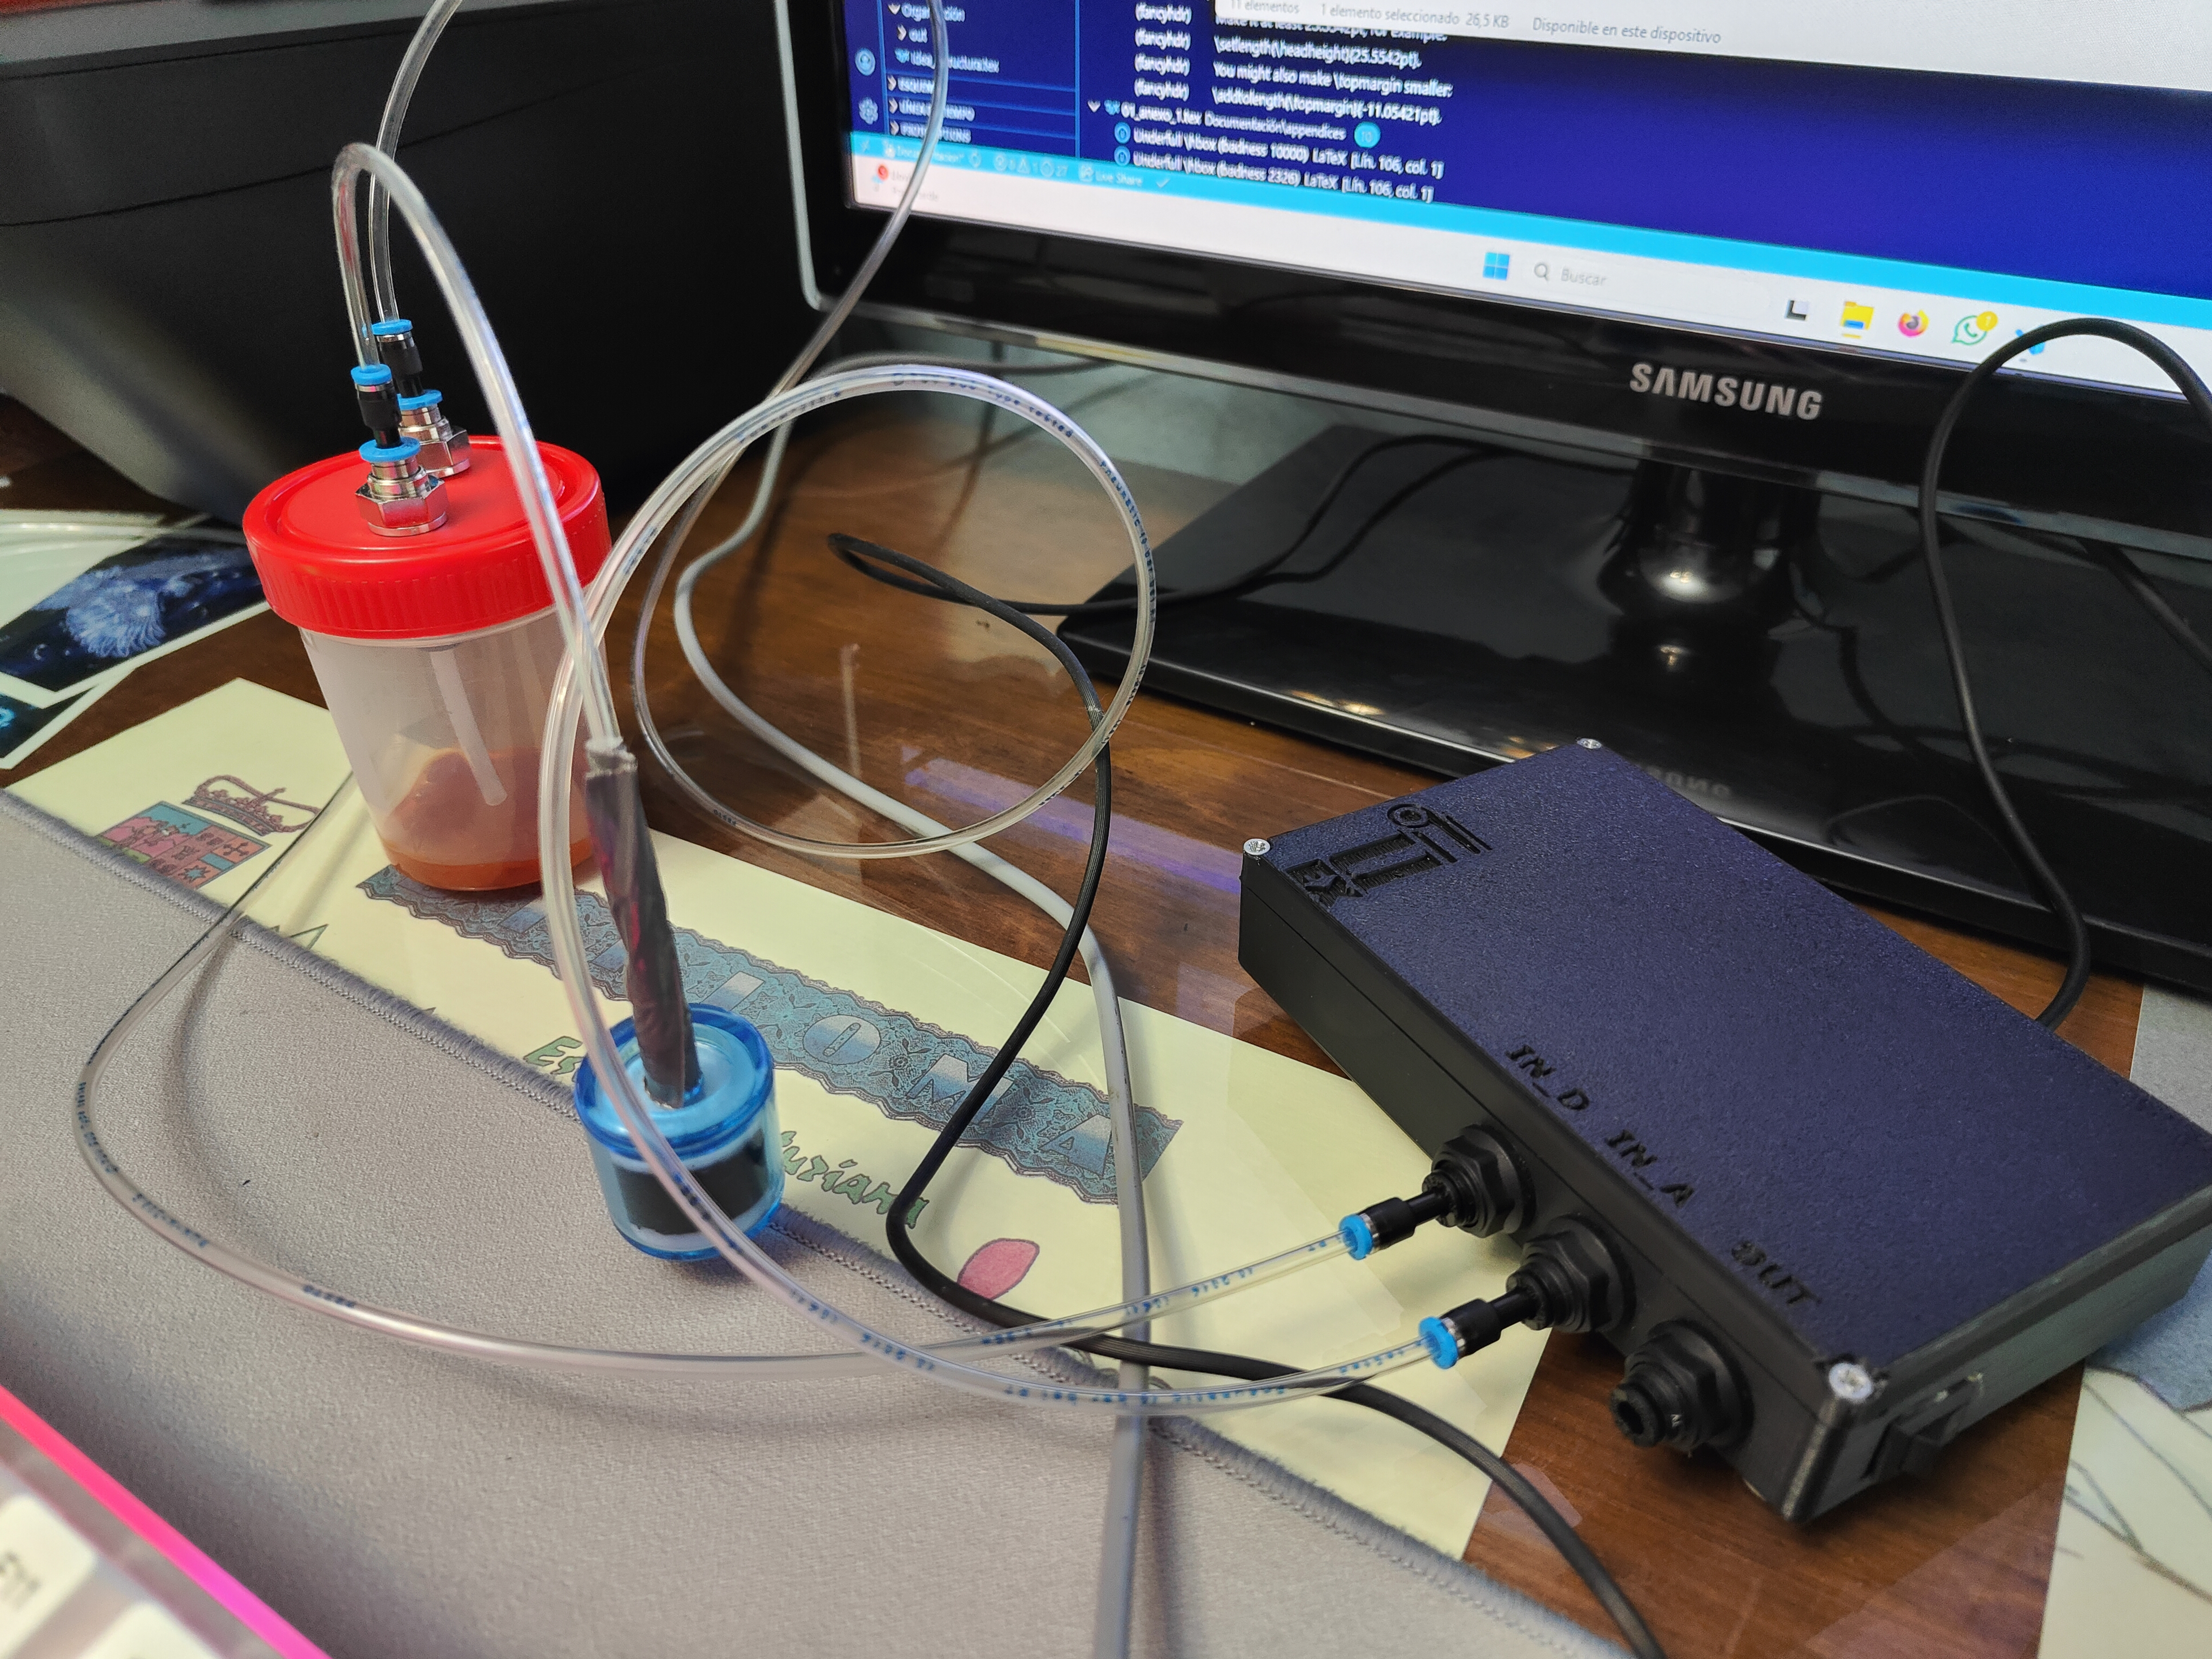
\includegraphics[width=0.65\textwidth]{pictures/Circuito_entero.jpg}
    \caption{Disposición del equipo para la muestra EXP\_M\_5--1.}\label{fig:setup_muestreo}
\end{figure}

Por otra parte, también es posible tomar muestras sin necesidad de usar el bote de muestreo, conectando directamente un tubo de adsorción que enctre en contacto con el aire, por ejemplo para tomar muestra de la calidad de aire de una habitación entera, o colocandolo cerca de una sustancia, como ocurre en la Figura~\ref{fig:setup_muestreo_sin_bote}.

\begin{figure}[H]
    \centering
    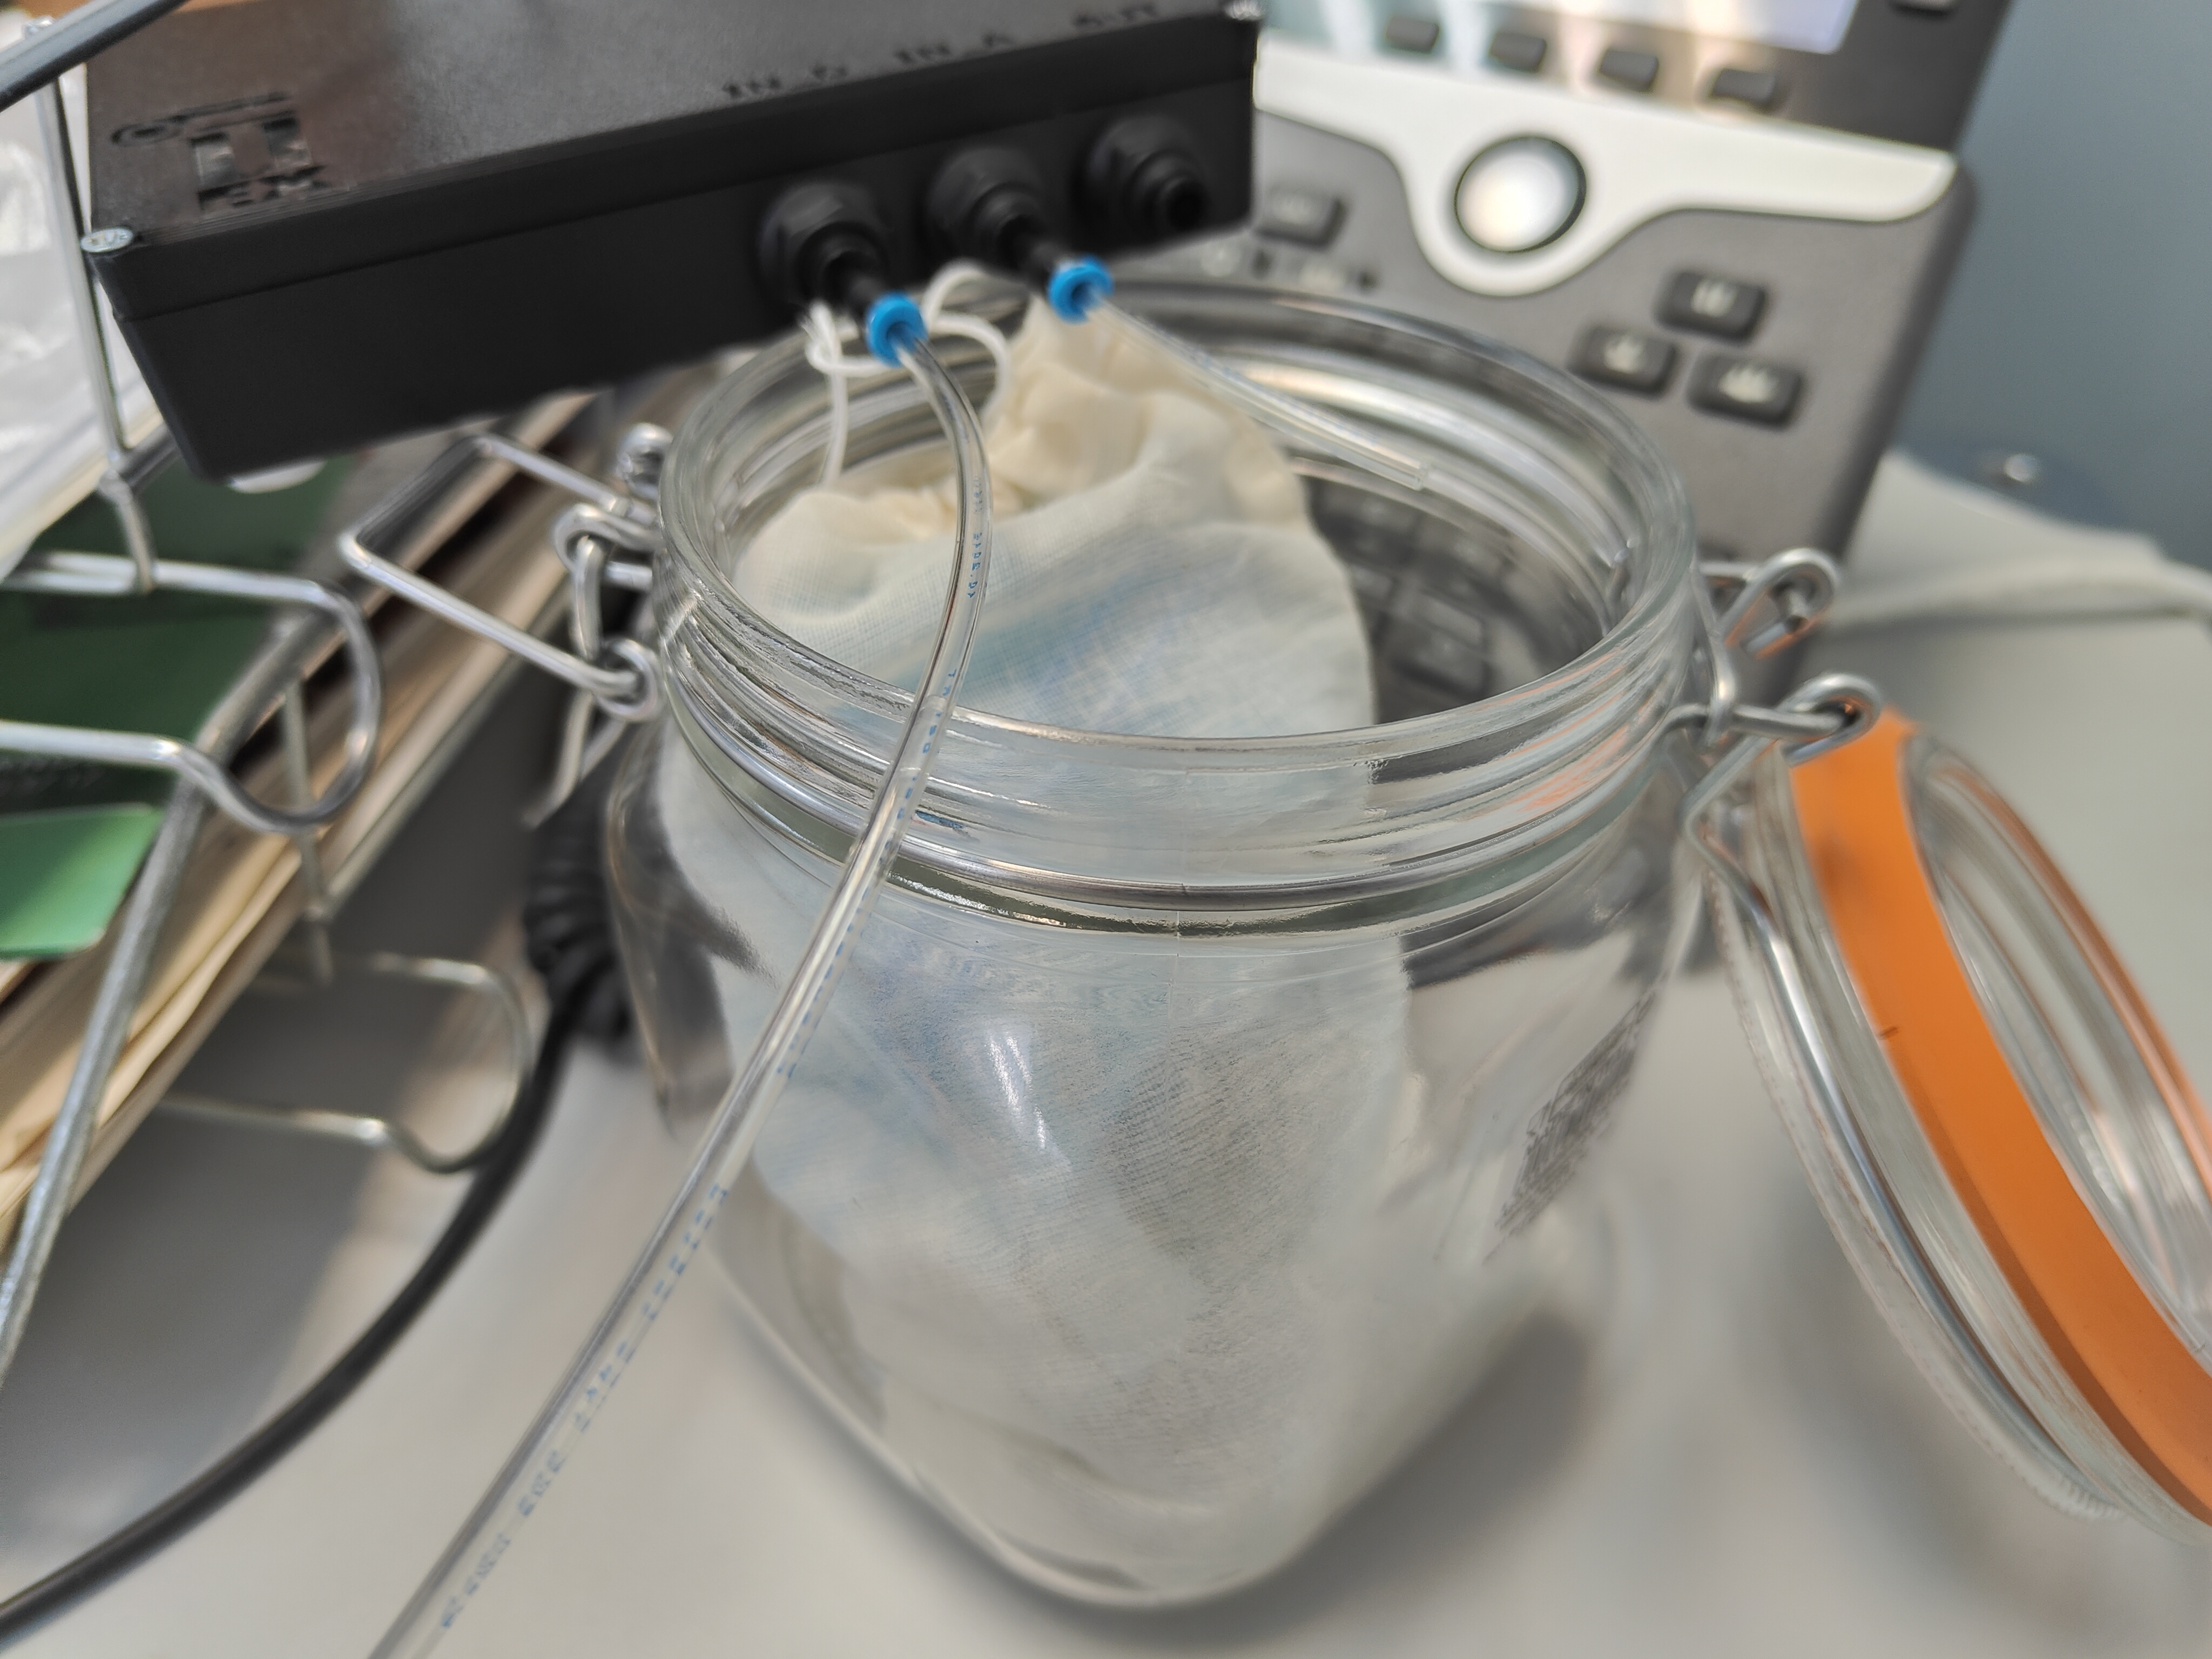
\includegraphics[width=0.65\textwidth]{pictures/Circuito_abierto.jpg}
    \caption{Disposición del equipo para la muestra EXP\_B\_34.}\label{fig:setup_muestreo_sin_bote}
\end{figure}

Antes de poder empezar a tomar muestras, es imprescidible encender la nariz electrónica con una hora o 45 minutos de antelación para que los sensores se estabilicen térmicamente y las lecturas sean fiables.
\par

Una vez los sensores se han calentado y la sustancia está preparada, solo queda conectar la nariz electrónica a un telefono movil android mediante Bluetooth y usar la aplicación móvil desarrollada para controlar la toma de muestras. Habría que configurar en número de ciclos y los tiempos de adsorción y desorción en las condiciones que se han mencionado anteriormente (1 ciclo, 120 segundos de desorción y 300 segundos de adsorción) y ya podría iniciarse la toma de muestras enviando el comando a través de la aplicación. Para saber como configurar la aplicación y conectarla a la nariz electrónica, se puede consultar el Anexo 3.
\par

Una vez haya finalizado la toma de la muestra, los datos se habrán al macenado en un fichero de texto llamado ``DATOS.txt'' en la tarjeta SD de la nariz electrónica. El siguiente paso es copiar este fichero al ordenador y cambiarle el nombre por el correspondiente a la nomenclatura mencionada anteriormente. Es importante borrar el contenido de la tarjeta SD antes de iniciar una nueva toma de muestras. De no hacerse, los datos de la siguiente muestra se añadirán al final del fichero ``DATOS.txt''.

\subsubsection{Muestras negativas}

\subsubsection{Muestras positivas}

\subsubsection{Limpieza del dataset}
Todos los archivos de texto de las muestras se han ido guardando en una carpeta llamada \texttt{Por\_procesar}, en la que tambien se encuentran divididas en las subcarpetas ``BUENO'' y ``MALO''. Estos archivos cuentan con datos, como la presión o la humedad, que no son útiles para el entrenamiento de la ANN, por lo que se ha llevado a cabo un proceso de limpieza y preprocesamiento de los datos para eliminar información irrelevante y preparar los datos para su uso en el entrenamiento de la red neuronal.
\par

Este proceso de limpieza se realiza con un script en Python llamado \texttt{Limpiador.py}, que inspecciona cada archivo de texto en las carpetas \texttt{Entrenamiento/Por\_procesar/BUENO} y \texttt{Entrenamiento/Por\_procesar/MALO}, extrae únicamente las columnas correspondientes a las lecturas de los sensores relevantes para el análisis y elimina las filas de la fase de desorción para solo tener datos de la fase de adsorción. Los archivos limpios se guardan en nuevas carpetas llamadas \texttt{Entrenamiento/BUENO} y \texttt{Entrenamiento/MALO} respectivamente, manteniendo la misma estructura de nombres de archivo para facilitar su identificación.

\subsection{Entrenamiento de la red neuronal}

\subsection{Desarrollo de la aplicación móvil}